\documentclass[12pt]{article}

% Language setting
% Replace `english' with e.g. `spanish' to change the document language
\usepackage[utf8]{inputenc} % Включаем поддержку UTF8
\usepackage[russian]{babel} % Включаем пакет для поддержки русского языка
	

% Set page size and margins
% Replace `letterpaper' with `a4paper' for UK/EU standard size
\usepackage[letterpaper,top=2cm,bottom=2cm,left=3cm,right=3cm,marginparwidth=1.75cm]{geometry}

% Useful packages
\usepackage{amsmath}
\usepackage{graphicx}
\usepackage[colorlinks=true, allcolors=blue]{hyperref}

\title{Эссе по защите информации}
\title{Алгоритмы Bear, Lion}
\author{Радюш Дарья, Б01-906}

\begin{document}
\maketitle



\section{Введение}

Известно множество алгоритмов симметричного шифрования, полученных путем разделения на раунды и использования в каждом раунде одного и того же алгоритма шифрования с различными преобразованиями или же путём многократного повторения конкретного алгоритма. Первый из этих вариантов не нашёл широкого применения из-за низкой скорости ($xDES^{3}$), примерами второго можно назвать Double DES, Triple DES. Использовать в алгоритмах блочного симметричного шифрования другие типы криптографических преобразований предложили в 1988 г. Одним из воплощений этой идеи и являются алгоритмы Bear и Lion.  

Блочные шифры Bear и Lion были предложены профессором Россом Андерсоном и криптоаналитиком Эли Бихамом в 1995г. Они созданы путём объединения алгоритма генерации псевдослучайных чисел с криптографической хэш-функцией. Bear дважды использует хэш-функцию с независимыми ключами и один раз -- поточный шифр с генератором псевдослучайных ключей. Lion использует поточный шифр дважды и хэш-функцию один раз. Доказано, что два этих алгоритма являются безопасными в том смысле, что атаки, которые восстанавливают ключи, по итогу сломают один или оба базовых компонента.  Bear и Lion также можно считать намного быстрее существующих блочных шифров. В данной работе рассматривается структура и криптоанализ этих алгоритмов.

\section{Bear}

Как уже говорилось, алгоритм Bear использует два хэша и один поточный шифр. Рассмотрим подробнее.

Пусть блоки входных данных больших размеров (примерно 1Кбайт-1Мбайт) и m (бит) - размер блока. ${H_{K}(M)}$ - хэш-функция с ключом K для сообщения M произвольной длины, результат которой фиксированный размер k бит. В качестве хэш-функции авторы алгоритмов предлагают использовать SHA-1 или MD5 (k = 160 для SHA-1 и k = 128 для MD5). Эти алгоритмы хэширования являются бесключевыми, однако предлагается вставлять ключ до и после хэшируемых данных (${\cdot}$ - операция конкатенации):
                 \[H_{k1}(M) = {MD5(k1\cdot M \cdot k1)}\]
                  
Далее пусть S(M) - поточный шифр или, более формально, псевдослучайная функция, которая при вводе M сгенерирует выходные данные произвольной длины.

Открытый текст P разделён на левую L и правую R части, размеры которых равны $|L| = k$, $|R| = m - k$. Ключ состоит из двух подключей K = (k1, k2) одинакового размера $b$, $b > k$.

Шифрование выполняется следующим образом:
\[L = L\oplus H_{k1}(R)\]
\[R = R\oplus S(L)\]
\[L = L\oplus H_{k2}(R)\]

Расшифрование:
\[L = L\oplus H_{k2}(R)\]
\[R = R\oplus S(L)\]
\[L = L\oplus H_{k1}(R)\]


\begin{figure}
\centering
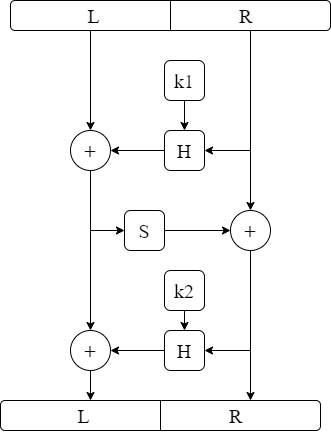
\includegraphics[width=0.3\textwidth]{Bear.png}
\caption{\label{fig:Bear}Алгоритм Bear.}
\end{figure}
\vspace{5mm}
Свойства хэш-функции $H_{k}(X) = {H'(k\cdot M \cdot k)}$:

    1) Является необратимой, так как при заданном $Y$ трудно найти $X$ такой, что $H'(X) = Y$;
   
    2) Уникальна для каждого значения, так как трудно найти неравные X и $Y$ такие, что $H'(X) = H'(Y)$;
    
    3) Является псевдослучайной, поскольку даже при заданном $H'(X_{i})$ для любого набора входных данных трудно предсказать какой-либо бит $H'(Y)$ для нового входного $Y$.
\vspace{5mm}

Свойства поточного шифра $S(M)$:

    1) Сопротивляется атакам восстановления ключа, поскольку трудно найти начальное $X$, учитывая $Y = S(X)$
    
    2) Сопротивляется атакам расширения, так как трудно расширить какой-либо частичный поток $Y$.

\section{Безопасность алгоритма Bear} 

Стоит рассмотреть теоремы, которые покажут, почему атаки восстановления ключа по итогу сломают как поточный шифр, так и хэш-функцию.    

\vspace{5mm}
\textbf{Теорема 1.} Оракул, который находит ключ алгоритма Bear по одной паре открытый текст/зашифрованный текст, может эффективно и с высокой вероятностью найти начальное значение $M$ поточного шифра $S$ для любого конкретного вывода $Y = S(M)$.

Доказательство. 

Учитывая $Y = S (M)$, мы хотим найти M. Мы генерируем открытый текст $P = (L, R)$
и зашифрованный текст $C = (L', R')$ такой, что $R \oplus R' = Y$, и такой, что L и L'
являются случайными. Поскольку мы предполагаем, что $|K1| = |K2| > k$, с высокой вероятностью
существуют некоторые значения $K1$ и $K2$, такие, что $H_{K1}(R) = L \oplus M$ и такие, что
$H_{K2}(R) = L' \oplus M$ (хотя M все еще неизвестно злоумышленнику). Используя
оракул, мы можем найти такие значения $K1$ и $K2$. Учитывая $K1$ и $K2$, мы можем легко
вывести $M$.

\vspace{5mm}
\textbf{Теорема 2.} Оракул, который находит ключ алгоритма Bear по одной паре открытый текст/зашифрованный текст, может эффективно и с высокой вероятностью находить прообразы и коллизии
хэш-функции $H$.

Доказательство. 

Вычислим выходные данные потокового шифра для входного 0: $Y_{0} = S(0)$.
Выберем случайное $R$ и установим $R' = R \oplus Y_{0}$. Установим $L = L' = 0$ и решим ключ для открытого текста $P = (L, R)$ и зашифрованного текста $C = (L', R')$. Учитывая этот ключ, мы фактически получаем два сообщения, оба из которых хэшируются до нулевого значения. Выбирая входные данные, отличные от нуля, мы можем получить произвольные прообразы.

\vspace{5mm}
Рассмотрим случай частичной атаки. Если мы можем расширить выходные данные поточного шифра (например, путём поиска входного ключа), то, учитывая зашифрованный текст и часть открытого текста, мы можем узнать больше информации об открытом тексте. С другой стороны, если для хэш-функции можно обнаружить коллизии, то злоумышленник может найти пары открытых текстов, правые половины которых имеют одинаковое значение, и, таким образом, сгенерировать зашифрованный текст, большинство битов которого предсказуемы.


\section{Lion}
Алгоритм Lion отличен от алгоритма Bear последовательностью использования функций H(R) и S(L), и фрагментов ключа шифрования. Lion, аналогично Bear, делит шифруемый блок на два субблока $L$ и $R$ различного размера: $b1$ и $b2$, которые выбираются аналогичным образом. Ключ шифрования делится на два подключа $k1$ и $k2$, размер каждого из которых равен $b1$.

\begin{figure}
\centering
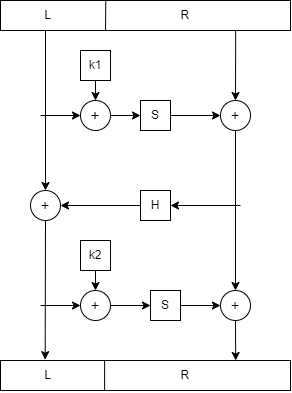
\includegraphics[width=0.3\textwidth]{Lion.png}
\caption{\label{fig:Lion}Алгоритм Lion.}
\end{figure}
\vspace{5mm}

\vspace{5mm}
Шифрование выполняется при помощи:
\[R = R\oplus S(L\oplus k1)\]
\[L = L\oplus H(R)\]
\[R = R\oplus S(L\oplus k2)\]

Расшифрование:
\[R = R\oplus S(L\oplus k2)\]
\[L = L\oplus H(R)\]
\[R = R\oplus S(L\oplus k1)\]

\vspace{5mm}
В этом случае мы можем иметь более слабое предположение о хэш-функции. Нам не
нужно предполагать, что это псевдослучайная функция, а просто то, что она
свободна от столкновений, т.е. что трудно найти различные $X1$, $X2$ такие, что $H'(X1) = H'(X2)$. Потоковый шифр $S(M)$ в этом случае таков: 

 1) Сопротивляется атакам восстановления ключа;
    
 2) Сопротивляется атакам расширения;

 3) Является псевдослучайной.

\vspace{5mm}
Снижение безопасности Lion происходит аналогично снижению безопасности Bear; оракул, который находит ключ алгоритма, разрушит обе его компоненты. Частичные атаки также сокращаются, и, например, мы обнаруживаем, что если злоумышленник знает прообраз 0 в хэш-функции, то мы получаем набор слабых ключей; везде, где $K1 = K2$, определенные открытые тексты будут зашифрованы для самих себя. 


\section{Производительность алгоритмов}
Рассмотренные выше алгоритмы были протестированы, используя блоки различных размеров. Была использована машину DEC Alpha с частотой 133 МГц с SHA1 в качестве хэш-функции и SEAL(симметричный поточный алгоритм шифрования данных, который оптимизирован для программной реализации) в качестве потокового шифрования.

Хэш-функция SHA1 была введена в Bear с помощью $H_{k}(M) = {H(k1\cdot M \cdot k1)}$; потоковый шифр $S(M) = SEAL_{M}(0) - SEAL_{M}(1) - SEAL_{M}(2) - ... - SEAL_{M}([m/(64*1024*8)])$.

Было обнаружено, что, несмотря на рекламируемые скорости 41,51 Мбит/сек для SHA1 и 114,8 Мбит/сек для SEAL на DEC Alpha с частотой 133 МГц, была получена скорость для BEAR всего около 13 Мбит/сек. Это несколько варьировалось в зависимости от размера блока, от 12,95 Мбит/сек для блоков размером 64 КБ до 13,62 Мбит/сек для блоков размером 1 МБ, что говорит о том, что время настройки ключа для SEAL было значительным. LION подтвердил это; вместо того, чтобы быть значительно быстрее, он работал со скоростью от 14,83 Мбит/сек для блоков размером 64 КБ до 18,68 Мбит/сек для блоков размером 1 МБ. Также проводилось тестирование SEAL для различных размеров блоков; обнаружено, что при включенной настройке ключа он работает на 58,7 Мбит/сек с блоками по 64 КБ и всего 7,6 Мбит/сек с блоками по 4096 байт - это далеко от заявленной производительности. 

На актуальных конфигурациях (процессоры Intel 10 поколения и выше с частотой от 3ГГц) скорость алгоритма Bear в среднем 32 Мбайт/сек, а алгоритма Lion 145 Мбайт/сек для блоков размером 64 КБ.

Эти результаты показывают необходимость в потоковом шифре, который быстро выполняется в программном
обеспечении, но не достигает этого за счет очень медленного расписания ключей. Учитывая такие шифры, ожидается, что BEAR и LION будут очень конкурентоспособны как быстрые блочные шифры.

\section{Lioness}

Авторы алгоритма предположили, что Lion может быть подвержен сложной в реализации комбинированной атаке на основе адаптивного выбора открытого текста и шифртекста. Поэтому был предложен более сложный алгоритм шифрования Lioness, не подверженный подобной атаке. В отличие от «трехраундовых» Bear и Lion, преобразования алгоритма
Lioness выполняются в 4 раунда, что и делает алгоритм более сложным и, соответсвенно, более медленный.

В каждом раунде Lioness используется один из независимых подключей алгоритма $k1...k4$. 

Шифрование выполняется следующим образом:
\[R = R\oplus S(L\oplus k1)\]
\[L = L\oplus H_{k2}(R)\]
\[R = R\oplus S(L\oplus k3)\]
\[L = L\oplus H_{k4}(R)\]
\newpage
Расшифрование выполняется применением обратной последовательности операций:
\[L = L\oplus H_{k4}(R)\]
\[R = R\oplus S(L\oplus k3)\]
\[L = L\oplus H_{k2}(R)\]
\[R = R\oplus S(L\oplus k1)\]

Алгоритм Lioness является по своей сути комбинацией преобразований алгоритмов Bear и Lion. Подключи $k2$ и $k4$ имеют произвольный размер (аналогично Bear), больший значения $b1$, а подключи $k1$ и $k3$ имеют размер $b1$ (аналогично Lion).

\vspace{5mm}
\begin{figure}
\centering
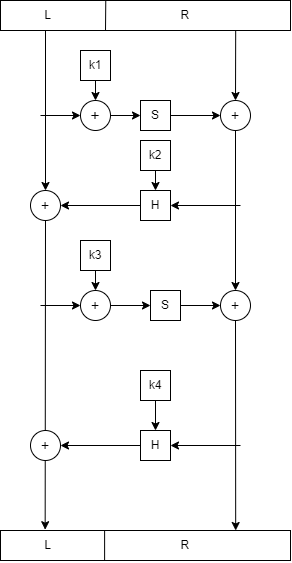
\includegraphics[width=0.3\textwidth]{Lioness.png}
\caption{\label{fig:Lioness}Алгоритм Lioness.}
\end{figure}

\section{Режимы работы}
Авторы предлагают использовать вышеуказанные шифры со следующими режимами работы:

\vspace{5mm}
1. Шифрование одного блока: все сообщение обрабатывается как один блок.
Этот режим имеет несколько преимуществ: 

(а) Каждый бит зашифрованного текста зависит от всех битов открытого текста очень сложным образом, что повышает криптографическую надежность; 

(б) Доказательства безопасности Bear и Lion сохраняются, поскольку только один блок зашифрован любым ключом; 

(в) Он предотвращает как дифференциальные, так и линейные атаки, поскольку злоумышленник не может получить более одного блока, зашифрованного одним и тем же ключом.

2. Сообщение может быть разделено на несколько блоков, и каждый блок зашифрован
под другим ключом.

3. Lioness также можно использовать со стандартными режимами шифрования DES: можно разделить сообщение на несколько блоков некоторой длины (скажем, 1Кбайт-1Мбайт) и использовать стандартные режимы DES. (DES — алгоритм для симметричного шифрования, утверждённый в 1977 году как официальный стандарт)

\vspace{5mm}
Режимы работы, блоки которых являются длинными и/или переменными, могут иметь дополнительные преимущества в конкретных областях применения. Например, при построении протоколов аутентификации использование блочного шифра переменной длины, который обрабатывает каждое сообщение протокола как отдельный блок, предотвратит атаки сращивания, подобные тем, которые были продемонстрированы в реализациях DES-CBC протокола Otway-Rees [MB94]. Другим примером является случай, когда требуется, чтобы все биты сеансового ключа, кроме 40 бит, отправлялись в открытом виде; если кто-то хочет получить максимально достижимый уровень безопасности с учетом этого ограничения, то использование большего блока заставляет криптоаналитика работать усерднее.

\section{Заключение}
Ранее уже было известно, как построить потоковые шифры и хэш-функции
из блочных шифров, а хэш-функции из потоковых шифров; показав, как
построить блочный шифр из потокового шифра и хэш-функции, авторы
завершили набор элементарных сокращений. 

Стоит отметить, что Bear, Lion и Lioness являются шаблонными конструкциями, так как не конкретизируют основные исользуемые параметры. Эти конструкции обладают некоторыми интересными доказуемыми свойствами безопасности, а также могут иметь практическую ценность: они обеспечивают быстроту и надежность блочных шифров, размеры блоков которых велики и изменчивы. Рассмотренные алгоритмы можно было значительно ускорить за счёт разработки поточного шифра с меньшим временем настройки ключа. Это является предметом продолжающихся исследований.


\bibliographystyle{alpha}
\bibliography{sample}


1. \url{https://www.phantastike.com/encryption/algoritmy_shifrovaniya/djvu/view/}

2. \url{https://ru.wikibrief.org/wiki/BEAR_and_LION_ciphers}

3. \url{https://www.cl.cam.ac.uk/~rja14/Papers/bear-lion.pdf}

4. \url{https://ru.wikipedia.org/wiki/SEAL_(криптографический_алгоритм)}

\end{document}
